% Options for packages loaded elsewhere
\PassOptionsToPackage{unicode}{hyperref}
\PassOptionsToPackage{hyphens}{url}
\PassOptionsToPackage{dvipsnames,svgnames,x11names}{xcolor}
%
\documentclass[
  11pt,
  a4paper,
]{article}

\usepackage{amsmath,amssymb}
\usepackage{iftex}
\ifPDFTeX
  \usepackage[T1]{fontenc}
  \usepackage[utf8]{inputenc}
  \usepackage{textcomp} % provide euro and other symbols
\else % if luatex or xetex
  \usepackage{unicode-math}
  \defaultfontfeatures{Scale=MatchLowercase}
  \defaultfontfeatures[\rmfamily]{Ligatures=TeX,Scale=1}
\fi
\usepackage[]{libertinus}
\ifPDFTeX\else  
    % xetex/luatex font selection
    \setmonofont[Scale=0.92]{Latin Modern Mono}
\fi
% Use upquote if available, for straight quotes in verbatim environments
\IfFileExists{upquote.sty}{\usepackage{upquote}}{}
\IfFileExists{microtype.sty}{% use microtype if available
  \usepackage[]{microtype}
  \UseMicrotypeSet[protrusion]{basicmath} % disable protrusion for tt fonts
}{}
\makeatletter
\@ifundefined{KOMAClassName}{% if non-KOMA class
  \IfFileExists{parskip.sty}{%
    \usepackage{parskip}
  }{% else
    \setlength{\parindent}{0pt}
    \setlength{\parskip}{6pt plus 2pt minus 1pt}}
}{% if KOMA class
  \KOMAoptions{parskip=half}}
\makeatother
\usepackage{xcolor}
\usepackage[a4paper,textheight=24cm,textwidth=15.5cm]{geometry}
\setlength{\emergencystretch}{3em} % prevent overfull lines
\setcounter{secnumdepth}{5}
% Make \paragraph and \subparagraph free-standing
\makeatletter
\ifx\paragraph\undefined\else
  \let\oldparagraph\paragraph
  \renewcommand{\paragraph}{
    \@ifstar
      \xxxParagraphStar
      \xxxParagraphNoStar
  }
  \newcommand{\xxxParagraphStar}[1]{\oldparagraph*{#1}\mbox{}}
  \newcommand{\xxxParagraphNoStar}[1]{\oldparagraph{#1}\mbox{}}
\fi
\ifx\subparagraph\undefined\else
  \let\oldsubparagraph\subparagraph
  \renewcommand{\subparagraph}{
    \@ifstar
      \xxxSubParagraphStar
      \xxxSubParagraphNoStar
  }
  \newcommand{\xxxSubParagraphStar}[1]{\oldsubparagraph*{#1}\mbox{}}
  \newcommand{\xxxSubParagraphNoStar}[1]{\oldsubparagraph{#1}\mbox{}}
\fi
\makeatother

\usepackage{color}
\usepackage{fancyvrb}
\newcommand{\VerbBar}{|}
\newcommand{\VERB}{\Verb[commandchars=\\\{\}]}
\DefineVerbatimEnvironment{Highlighting}{Verbatim}{commandchars=\\\{\}}
% Add ',fontsize=\small' for more characters per line
\newenvironment{Shaded}{}{}
\newcommand{\AlertTok}[1]{\textcolor[rgb]{1.00,0.33,0.33}{\textbf{#1}}}
\newcommand{\AnnotationTok}[1]{\textcolor[rgb]{0.42,0.45,0.49}{#1}}
\newcommand{\AttributeTok}[1]{\textcolor[rgb]{0.84,0.23,0.29}{#1}}
\newcommand{\BaseNTok}[1]{\textcolor[rgb]{0.00,0.36,0.77}{#1}}
\newcommand{\BuiltInTok}[1]{\textcolor[rgb]{0.84,0.23,0.29}{#1}}
\newcommand{\CharTok}[1]{\textcolor[rgb]{0.01,0.18,0.38}{#1}}
\newcommand{\CommentTok}[1]{\textcolor[rgb]{0.42,0.45,0.49}{#1}}
\newcommand{\CommentVarTok}[1]{\textcolor[rgb]{0.42,0.45,0.49}{#1}}
\newcommand{\ConstantTok}[1]{\textcolor[rgb]{0.00,0.36,0.77}{#1}}
\newcommand{\ControlFlowTok}[1]{\textcolor[rgb]{0.84,0.23,0.29}{#1}}
\newcommand{\DataTypeTok}[1]{\textcolor[rgb]{0.84,0.23,0.29}{#1}}
\newcommand{\DecValTok}[1]{\textcolor[rgb]{0.00,0.36,0.77}{#1}}
\newcommand{\DocumentationTok}[1]{\textcolor[rgb]{0.42,0.45,0.49}{#1}}
\newcommand{\ErrorTok}[1]{\textcolor[rgb]{1.00,0.33,0.33}{\underline{#1}}}
\newcommand{\ExtensionTok}[1]{\textcolor[rgb]{0.84,0.23,0.29}{\textbf{#1}}}
\newcommand{\FloatTok}[1]{\textcolor[rgb]{0.00,0.36,0.77}{#1}}
\newcommand{\FunctionTok}[1]{\textcolor[rgb]{0.44,0.26,0.76}{#1}}
\newcommand{\ImportTok}[1]{\textcolor[rgb]{0.01,0.18,0.38}{#1}}
\newcommand{\InformationTok}[1]{\textcolor[rgb]{0.42,0.45,0.49}{#1}}
\newcommand{\KeywordTok}[1]{\textcolor[rgb]{0.84,0.23,0.29}{#1}}
\newcommand{\NormalTok}[1]{\textcolor[rgb]{0.14,0.16,0.18}{#1}}
\newcommand{\OperatorTok}[1]{\textcolor[rgb]{0.14,0.16,0.18}{#1}}
\newcommand{\OtherTok}[1]{\textcolor[rgb]{0.44,0.26,0.76}{#1}}
\newcommand{\PreprocessorTok}[1]{\textcolor[rgb]{0.84,0.23,0.29}{#1}}
\newcommand{\RegionMarkerTok}[1]{\textcolor[rgb]{0.42,0.45,0.49}{#1}}
\newcommand{\SpecialCharTok}[1]{\textcolor[rgb]{0.00,0.36,0.77}{#1}}
\newcommand{\SpecialStringTok}[1]{\textcolor[rgb]{0.01,0.18,0.38}{#1}}
\newcommand{\StringTok}[1]{\textcolor[rgb]{0.01,0.18,0.38}{#1}}
\newcommand{\VariableTok}[1]{\textcolor[rgb]{0.89,0.38,0.04}{#1}}
\newcommand{\VerbatimStringTok}[1]{\textcolor[rgb]{0.01,0.18,0.38}{#1}}
\newcommand{\WarningTok}[1]{\textcolor[rgb]{1.00,0.33,0.33}{#1}}

\providecommand{\tightlist}{%
  \setlength{\itemsep}{0pt}\setlength{\parskip}{0pt}}\usepackage{longtable,booktabs,array}
\usepackage{calc} % for calculating minipage widths
% Correct order of tables after \paragraph or \subparagraph
\usepackage{etoolbox}
\makeatletter
\patchcmd\longtable{\par}{\if@noskipsec\mbox{}\fi\par}{}{}
\makeatother
% Allow footnotes in longtable head/foot
\IfFileExists{footnotehyper.sty}{\usepackage{footnotehyper}}{\usepackage{footnote}}
\makesavenoteenv{longtable}
\usepackage{graphicx}
\makeatletter
\def\maxwidth{\ifdim\Gin@nat@width>\linewidth\linewidth\else\Gin@nat@width\fi}
\def\maxheight{\ifdim\Gin@nat@height>\textheight\textheight\else\Gin@nat@height\fi}
\makeatother
% Scale images if necessary, so that they will not overflow the page
% margins by default, and it is still possible to overwrite the defaults
% using explicit options in \includegraphics[width, height, ...]{}
\setkeys{Gin}{width=\maxwidth,height=\maxheight,keepaspectratio}
% Set default figure placement to htbp
\makeatletter
\def\fps@figure{htbp}
\makeatother
% definitions for citeproc citations
\NewDocumentCommand\citeproctext{}{}
\NewDocumentCommand\citeproc{mm}{%
  \begingroup\def\citeproctext{#2}\cite{#1}\endgroup}
\makeatletter
 % allow citations to break across lines
 \let\@cite@ofmt\@firstofone
 % avoid brackets around text for \cite:
 \def\@biblabel#1{}
 \def\@cite#1#2{{#1\if@tempswa , #2\fi}}
\makeatother
\newlength{\cslhangindent}
\setlength{\cslhangindent}{1.5em}
\newlength{\csllabelwidth}
\setlength{\csllabelwidth}{3em}
\newenvironment{CSLReferences}[2] % #1 hanging-indent, #2 entry-spacing
 {\begin{list}{}{%
  \setlength{\itemindent}{0pt}
  \setlength{\leftmargin}{0pt}
  \setlength{\parsep}{0pt}
  % turn on hanging indent if param 1 is 1
  \ifodd #1
   \setlength{\leftmargin}{\cslhangindent}
   \setlength{\itemindent}{-1\cslhangindent}
  \fi
  % set entry spacing
  \setlength{\itemsep}{#2\baselineskip}}}
 {\end{list}}
\usepackage{calc}
\newcommand{\CSLBlock}[1]{\hfill\break\parbox[t]{\linewidth}{\strut\ignorespaces#1\strut}}
\newcommand{\CSLLeftMargin}[1]{\parbox[t]{\csllabelwidth}{\strut#1\strut}}
\newcommand{\CSLRightInline}[1]{\parbox[t]{\linewidth - \csllabelwidth}{\strut#1\strut}}
\newcommand{\CSLIndent}[1]{\hspace{\cslhangindent}#1}

\usepackage{tikz}
\usepackage{xcolor}
\usepackage{tabularx}
\usepackage{orcidlink}
\usepackage{lineno}
\usepackage{libertinus}
\usepackage{draftwatermark}

\makeatletter
\@ifpackageloaded{tcolorbox}{}{\usepackage[skins,breakable]{tcolorbox}}
\@ifpackageloaded{fontawesome5}{}{\usepackage{fontawesome5}}
\definecolor{quarto-callout-color}{HTML}{909090}
\definecolor{quarto-callout-note-color}{HTML}{0758E5}
\definecolor{quarto-callout-important-color}{HTML}{CC1914}
\definecolor{quarto-callout-warning-color}{HTML}{EB9113}
\definecolor{quarto-callout-tip-color}{HTML}{00A047}
\definecolor{quarto-callout-caution-color}{HTML}{FC5300}
\definecolor{quarto-callout-color-frame}{HTML}{acacac}
\definecolor{quarto-callout-note-color-frame}{HTML}{4582ec}
\definecolor{quarto-callout-important-color-frame}{HTML}{d9534f}
\definecolor{quarto-callout-warning-color-frame}{HTML}{f0ad4e}
\definecolor{quarto-callout-tip-color-frame}{HTML}{02b875}
\definecolor{quarto-callout-caution-color-frame}{HTML}{fd7e14}
\makeatother
\makeatletter
\@ifpackageloaded{caption}{}{\usepackage{caption}}
\AtBeginDocument{%
\ifdefined\contentsname
  \renewcommand*\contentsname{Table of contents}
\else
  \newcommand\contentsname{Table of contents}
\fi
\ifdefined\listfigurename
  \renewcommand*\listfigurename{List of Figures}
\else
  \newcommand\listfigurename{List of Figures}
\fi
\ifdefined\listtablename
  \renewcommand*\listtablename{List of Tables}
\else
  \newcommand\listtablename{List of Tables}
\fi
\ifdefined\figurename
  \renewcommand*\figurename{Figure}
\else
  \newcommand\figurename{Figure}
\fi
\ifdefined\tablename
  \renewcommand*\tablename{Table}
\else
  \newcommand\tablename{Table}
\fi
}
\@ifpackageloaded{float}{}{\usepackage{float}}
\floatstyle{ruled}
\@ifundefined{c@chapter}{\newfloat{codelisting}{h}{lop}}{\newfloat{codelisting}{h}{lop}[chapter]}
\floatname{codelisting}{Listing}
\newcommand*\listoflistings{\listof{codelisting}{List of Listings}}
\usepackage{amsthm}
\theoremstyle{plain}
\newtheorem{theorem}{Theorem}[section]
\theoremstyle{remark}
\AtBeginDocument{\renewcommand*{\proofname}{Proof}}
\newtheorem*{remark}{Remark}
\newtheorem*{solution}{Solution}
\newtheorem{refremark}{Remark}[section]
\newtheorem{refsolution}{Solution}[section]
\makeatother
\makeatletter
\makeatother
\makeatletter
\@ifpackageloaded{caption}{}{\usepackage{caption}}
\@ifpackageloaded{subcaption}{}{\usepackage{subcaption}}
\makeatother
\makeatletter
\@ifpackageloaded{algorithm}{}{\usepackage{algorithm}}
\makeatother
\makeatletter
\@ifpackageloaded{algpseudocode}{}{\usepackage{algpseudocode}}
\makeatother
\makeatletter
\@ifpackageloaded{caption}{}{\usepackage{caption}}
\makeatother

\ifLuaTeX
  \usepackage{selnolig}  % disable illegal ligatures
\fi
\usepackage{bookmark}

\IfFileExists{xurl.sty}{\usepackage{xurl}}{} % add URL line breaks if available
\urlstyle{same} % disable monospaced font for URLs
\hypersetup{
  pdftitle={Reservoir Computing in R: a Tutorial for Using reservoirnet to Predict Complex Time-Series},
  pdfauthor={Thomas Ferté; Kalidou Ba; Dan Dutartre; Pierrick Legrand; Vianney Jouhet; Romain Griffier; Rodolphe Thiébaut; Xavier Hinaut; Boris Hejblum},
  pdfkeywords={Genetic algorithm, Reservoir Computing, High
dimension, Covid-19, Electronic Health Records, Time series},
  colorlinks=true,
  linkcolor={blue},
  filecolor={Maroon},
  citecolor={Blue},
  urlcolor={Blue},
  pdfcreator={LaTeX via pandoc}}


\title{Reservoir Computing in R: a Tutorial for Using reservoirnet to
Predict Complex Time-Series}
\author{Thomas Ferté \and Kalidou Ba \and Dan Dutartre \and Pierrick
Legrand \and Vianney Jouhet \and Romain Griffier \and Rodolphe
Thiébaut \and Xavier Hinaut \and Boris Hejblum}
\date{2024-11-20}

\begin{document}
\definecolor{computo-blue}{HTML}{034E79}

\begin{tikzpicture}[remember picture,overlay]
\fill[computo-blue]
  (current page.north west) -- (current page.north east) --
  ([yshift=-5cm]current page.north east|-current page.north east) --
  ([yshift=-5cm]current page.north west|-current page.north west) -- cycle;
\node[anchor=north west, xshift=.75cm,
  yshift=-.75cm] at (current page.north west) {\includegraphics[height=3cm]{logo_text_white}};
\node[font=\sffamily\bfseries\color{white},anchor=north west, xshift=.75cm,
  yshift=-4.25cm] at (current page.north
  west) {\fontsize{10}{12}\selectfont ISSN 2824-7795};
\node[font=\sffamily\bfseries\color{white},anchor=west,
  xshift=4.25cm,yshift=-2.75cm] at (current page.north west)
  {\begin{minipage}{15cm}
    \fontsize{25}{30}\selectfont
    Reservoir Computing in R: a Tutorial for Using reservoirnet to
    Predict Complex Time-Series
    \vspace{.5cm}
    \\
    \fontsize{15}{18}\selectfont
    
  \end{minipage}};
\end{tikzpicture}

\vspace*{2.5cm}
\begin{center}
          Thomas Ferté~\orcidlink{0000-0001-8455-4665}\quad
             Inserm Bordeaux Population Health Research Center UMR 1219,
Inria BSO, team SISTM, F-33000 Bordeaux, France, Inserm\\
              Inserm Bordeaux Population Health Research Center UMR
1219, Inria BSO, team SISTM, F-33000 Bordeaux, France, Inria\\
              Bordeaux Hospital University Center, Pôle de santé
publique, Service d'information médicale, F-33000 Bordeaux, France, CHU
de Bordeaux\\
                 Kalidou Ba~\orcidlink{0000-0001-6552-265X}\quad
             Inserm Bordeaux Population Health Research Center UMR 1219,
Inria BSO, team SISTM, F-33000 Bordeaux, France, Inserm\\
              Inserm Bordeaux Population Health Research Center UMR
1219, Inria BSO, team SISTM, F-33000 Bordeaux, France, Inria\\
              Bordeaux Hospital University Center, Pôle de santé
publique, Service d'information médicale, F-33000 Bordeaux, France, CHU
de Bordeaux\\
                 Dan Dutartre~\orcidlink{0000-0001-8210-461X}\quad
             Inria BSO, Inria\\
                 Pierrick Legrand\quad
             Inria BSO, F-33000 Bordeaux, France, Inria\\
              IMB, Institut de Mathématiques de Bordeaux, UMR CNRS
5251, IMB\\
                 Vianney Jouhet~\orcidlink{0000-0001-5272-2265}\quad
             Inserm Bordeaux Population Health Research Center UMR 1219,
team AHeaD, F-33000 Bordeaux, Inserm\\
              Bordeaux Hospital University Center, Pôle de santé
publique, Service d'information médicale, F-33000 Bordeaux, France, CHU
de Bordeaux\\
                 Romain Griffier~\orcidlink{0000-0002-1096-137X}\quad
             Inserm Bordeaux Population Health Research Center UMR 1219,
team AHeaD, F-33000 Bordeaux, Inserm\\
              Bordeaux Hospital University Center, Pôle de santé
publique, Service d'information médicale, F-33000 Bordeaux, France, CHU
de Bordeaux\\
                 Rodolphe Thiébaut~\orcidlink{0000-0002-5235-3962}\quad
             Inserm Bordeaux Population Health Research Center UMR 1219,
Inria BSO, team SISTM, F-33000 Bordeaux, France, Inserm\\
              Inserm Bordeaux Population Health Research Center UMR
1219, Inria BSO, team SISTM, F-33000 Bordeaux, France, Inria\\
              Bordeaux Hospital University Center, Pôle de santé
publique, Service d'information médicale, F-33000 Bordeaux, France, CHU
de Bordeaux\\
                 Xavier Hinaut~\orcidlink{0000-0002-1924-1184}\quad
             Inria BSO, F-33000 Bordeaux, France, Inria\\
              Univ. Bordeaux, CNRS, IMN, UMR 5293, Bordeaux,
France, CNRS\\
              LaBRI, Univ. Bordeaux, Bordeaux INP, CNRS UMR
5800., LaBRI\\
                 Boris
Hejblum~\orcidlink{0000-0003-0646-452X}\footnote{Corresponding author: }\quad
             Inserm Bordeaux Population Health Research Center UMR 1219,
Inria BSO, team SISTM, F-33000 Bordeaux, France, Inserm\\
              Inserm Bordeaux Population Health Research Center UMR
1219, Inria BSO, team SISTM, F-33000 Bordeaux, France, Inria\\
           
  \bigskip
  
  Date published: 2024-11-20 \quad Last modified: 2024-11-20
\end{center}
      
\bigskip
\begin{abstract}
Reservoir Computing (RC) is a machine learning method based on neural
networks that efficiently process information generated by dynamical
systems. It has been successful in solving various tasks including time
series forecasting, language processing or voice processing. RC is
implemented in Python and Julia but not in R. This article introduces
reservoirnet, an R package providing access to the Python API
ReservoirPy, allowing R users to harness the power of reservoir
computing. This article provides an introduction to the fundamentals of
RC and showcases its real-world applicability through three distinct
sections. First, we cover the foundational concepts of RC, setting the
stage for understanding its capabilities. Next, we delve into the
practical usage of reservoirnet through two illustrative examples. These
examples demonstrate how it can be applied to real-world problems,
specifically, regression of COVID-19 hospitalizations and classification
of Japanese vowels. Finally, we present a comprehensive analysis of a
real-world application of reservoirnet, where it was used to forecast
COVID-19 hospitalizations at Bordeaux University Hospital using public
data and electronic health records.
\end{abstract}

\noindent%
{\it Keywords:} Genetic algorithm, Reservoir Computing, High
dimension, Covid-19, Electronic Health Records, Time series
\vfill

\linenumbers
\DraftwatermarkOptions{stamp=true, colorspec=0.9, text={\rm submitted}}

\floatname{algorithm}{Algorithm}

\renewcommand*\contentsname{Contents}
{
\hypersetup{linkcolor=}
\setcounter{tocdepth}{3}
\tableofcontents
}

\section{Introduction}\label{introduction}

Reservoir Computing (RC) is a prominent machine learning method,
proposed by Jaeger (2001), Maass, Natschläger, and Markram (2002) and
Lukoševičius and Jaeger (2009) that has gained significant attention in
recent years for its ability to efficiently process information
generated by dynamical systems. This innovative approach leverages the
dynamics of a high-dimensional ``reservoir'' (we define it below) to
perform complex computations and solve various tasks based on the
response of this dynamical system to input signals. RC has demonstrated
its efficacy in tackling various challenges, encompassing pattern
classification and time series forecasting in applications ranging from
electrocardiogram analysis to bird calls Trouvain and Hinaut (2021),
language processing Hinaut and Dominey (2013), power plants, internet
traffic, stock prices, and beyond Lukoševičius and Jaeger (2009).

Originally, the RC paradigm was implemented in artificial firing-rate
neurons (``Echo State Networks'', Jaeger (2001)) and spiking neurons
(``Liquid State Machine'', Maass, Natschläger, and Markram (2002)) as a
recurrent neural network (RNN) where the internal recurrent connections,
denoted as the reservoir, are randomly generated and only the output
layer (named ``read-out'') is trained. The reservoir projects temporal
input signals onto a high-dimensional feature space facilitating the
learning of non-linear and temporal interactions. Thus, this recurrent
layer contains are high-dimensional non-linear recombination of the
inputs and past states: it is a ``reservoir of computations'' from which
useful information can be linearly extracted (or ``read-out'') to
provide the desired outputs. This offers the advantage of decreasing the
computing time while consistently maintaining robust performance
compared to conventional RNNs (Vlachas et al. 2020). In parallel, this
RC paradigm gained an increasing interest because of its ability to be
implemented not only on classical computers. Indeed, the hidden
recurrent layer can be kept untrained and thus a wide range of physical
media can be used to replace it. Recently, Tanaka et al. (2019) reviewed
this prolific field: from FPGA hardware (Penkovsky, Larger, and Brunner
2018), to spin waves using magnetic properties (Nakane, Tanaka, and
Hirose 2018), skrymions (Prychynenko et al. 2018) or optical
implementations (Rafayelyan et al. 2020). This provides interesting and
potentially more efficient alternative to traditional machine learning.

RC leverages various hyperparameters to introduce prior knowledge about
the relationship between input variables and output targets. However,
since the connections within the reservoir are randomly initialized, the
same set of hyperparameters may exhibit diverse behaviors across
different realizations of the reservoir connections. This
unpredictability makes it challenging to anticipate the performance of a
particular hyperparameter setting, as identical settings may produce
varying outcomes when applied to distinct instances of the reservoir.
Moreover, selecting the most suitable hyperparameters often requires
researchers to experiment with multiple combinations on a training
dataset and evaluate their performance on a separate test set. Although
this approach can be resource-intensive and time-consuming, it is a
compromise that is acceptable considering the rapid simulation
capabilities offered by RC.

\emph{XH : Commentaires généraux sur le paragraphe : il faut ne faut pas
insister sur les hyperparamètres comme si c'était négatif. Plutôt dire
qu'il y a des optimisations et tricks à connaitre, et que c'est
intéressant d'avoir une librairie pour ça, et aussi à des fins de
reproductibilité. Dire que c'est un trade-off car c'est les a priori
nécessaire qu'on rajoute dans l'algo car on gagne du temps sur
l'apprentissage. C'est ambigu de parler de stochaticité ici je trouve,
car le processus n'est pas stochastic une fois les poids fixés.}

\emph{TF : j'ai modifié, mieux ?}

The utilization of RC poses challenges on multiple fronts. Firstly, its
stochastic nature, attributed to the random aspect of the reservoir,
introduces unpredictability into the results, even with well-chosen
hyperparameters. Secondly, RC relies on numerous hyperparameters to
establish connections between neurons. Guidance on determining these
hyperparameters is limited, often requiring users to evaluate the
performance of different combinations of hyperparameters on a train set
before selecting the optimal combination to forecast on the test
set\footnote{In this article, we employ the term ``train set'' to refer
  to the combined dataset consisting of both the training and validation
  sets, which are cycled through in a cross-validation manner.}.
Thirdly, there is a current absence of implementation in R, rendering
the method challenging for users unfamiliar with Python (Trouvain and
Hinaut 2022) or Julia (Martinuzzi et al. 2022).

\emph{XH : Je pense que ça embrouille là : c'est train/test/validation
Les hyperparamètres sont entrainé sur le train set puis évalués sur le
validation set. Et ensuite le test set. Par abus de langage on dit
souvent « test set » au lieu de « validation set » quand on optimise les
paramètres. Moi ça me choque pas, mais dans un papier vaut mieux
utiliser les termes adéquats, ou en tous cas toujours utiliser les
memes, donc si tu n'as jamais de validation set (enfin le vrai test
set), ça peut passer (pas besoin de tout changer). Met juste une note de
bas de page pour préciser que en général on devrait l'appeler le
validation set. On verra ce que les reviewers disent, pas besoin de
perdre du temps maintenant.}

\emph{TF : ok, j'ai rajouté une note de bas de page ci-dessous}

In this paper, we endeavor to delve into these challenges, offering
comprehensive guidance to assist new users in maximizing the benefits of
RC. Initially, a broad introduction to reservoir computing is presented,
accompanied by a tutorial on its application using
\texttt{reservoirnet}, an R package built upon the \texttt{reservoirPy}
Python module Trouvain and Hinaut (2022). Subsequently, we investigate
the various challenges associated with the use of RC for forecasting
COVID-19 hospitalizations. This exploration includes detailed guidance
on the modeling strategy, the selection of hyperparameters, and the
implementation process.

\section{RC presentation}\label{rc-presentation}

RC is a machine learning paradigm which is most often implemented as
Echo State Networks (ESNs; Jaeger (2001)), the firing-rate neuron
version. An ESN is described by three matrices of connectivity: an input
layer \(W_{in}\), a recurrent layer \(W\) and an output layer
\(W_{out}\). At each time step, the input vector \(u_t\) is projected
into the reservoir which is also combined with reservoir past state
\(x(t-1)\) through the recurrent connections. The output \(y(t)\) is
linearly read-out from the reservoir. Input \(W_{in}\) and recurrent
\(W\) matrices are kept random; only the output matrix \(W_{out}\) is
trained in an offline or online method. Often a ridge regression (i.e.~a
regularized linear regression) is used to obtain the desired outputs
\(y(t)\) from the reservoir states \(x(t)\). Figure
@ref(fig:rcpresentation) depicts the architecture. For simplicity, we
will use the term ``reservoir computing'' for ``Echo State Network'' in
the remainder of the paper.

\begin{figure}[H]

{\centering 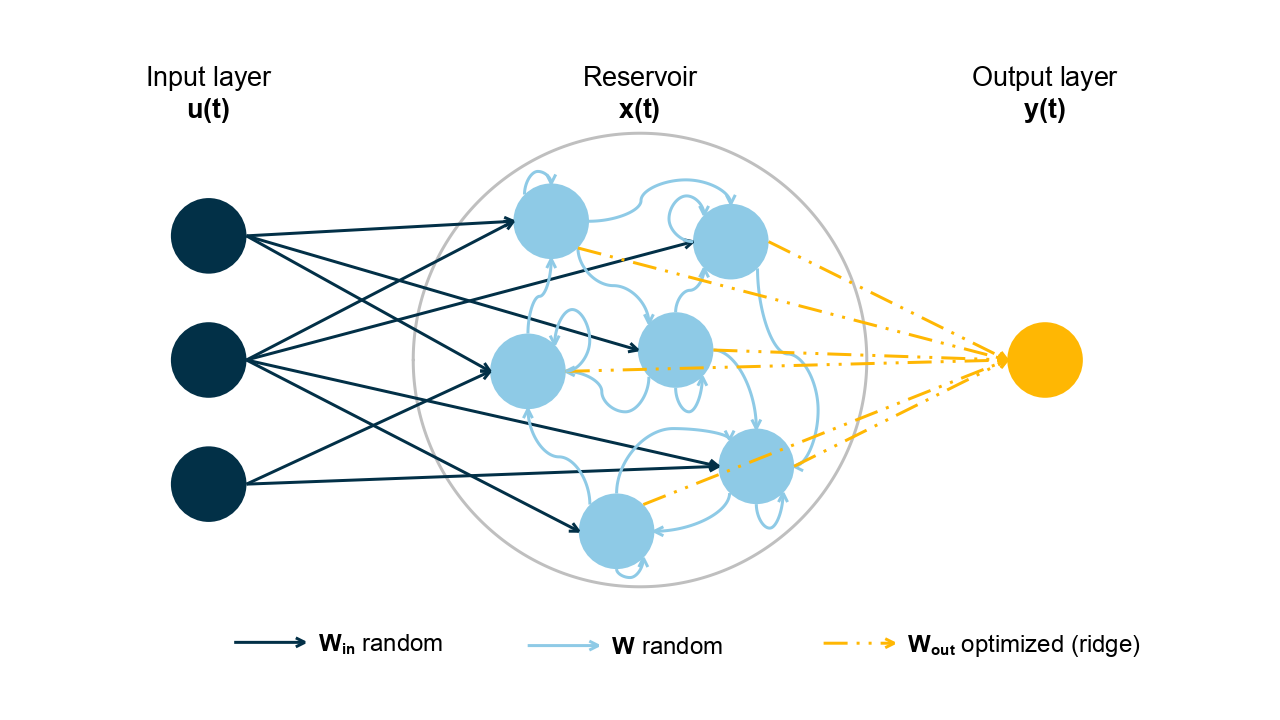
\includegraphics[width=0.9\textwidth,height=\textheight]{images/image1.png}

}

\caption{Reservoir computing is composed of an input layer, a reservoir
and an output layer. Connection between input layer and reservoir and
inside reservoir are random. Only the output layer is optimized based on
a ridge regression.}

\end{figure}%

The input layer \(u(t)\) is an \(M\)-dimension vector, where \(M\) is
the number of input time series, which corresponds to the values of the
input time series at time \(t\) where \(t = 1, …, T\). The reservoir
layer \(x(t)\) is an \(N_{res}\)-dimensional vector where \(N_{res}\) is
the number of nodes in the reservoir. The value \(x(t)\) is defined as
follow:

\[x( t+1 ) = ( 1 - \alpha )  x ( t) + \alpha \: tanh( W x(t) + W_{in} u(t+1) ) \text{ , where } \alpha \in [0, 1 ]\]

The leaking rate \(\alpha\) defines the rate of update of the nodes. The
closer \(\alpha\) is to \(1\), the higher the reservoir is sensitive to
new inputs (i.e \(u(t)\)). Therefore, the reservoir state at time
\(t+1\) denoted \(x(t+1)\) depends on the reservoir state at the
previous time (i.e \(x(t)\)) and the new inputs (i.e \(u(t+1)\)). Both
\(W_{in}\) and \(W\) are random matrices of size \(N_{res} \times M\)
and \(N_{res} \times N_{res}\) respectively.

The leaking rate \(\alpha\) defines the update rate of the nodes. The
closer \(\alpha\) is to \(1\), the more the reservoir is sensitive to
new inputs \(u(t)\). Therefore, the reservoir state at time \(t+1\)
denoted \(x(t+1)\) depends on the reservoir state at the previous time
\(x(t)\) and the new inputs \(u(t+1)\). Both \(W_{in}\) and \(W\) are
random matrices of size \(N_{res} \times M\) and
\(N_{res} \times N_{res}\) respectively.

\emph{XH : Ah tu utilises une matrice dense ? si oui, t'as fait ça dans
toutes tes simulations ? habituellement on utilise plutôt 10 ou 20\% de
connectivité, surtout si on prend un distribution bimodale comme
bernouilli. En tous cas il faut pas préciser que soit doit être dense
ici.}

\emph{TF : my bad, j'avais mal lu la doc. On utilise l'implémentation de
base de reservoirpy qui est effectivement sparse à 0.1 par défaut.}

\(W_{in}\) is a matrix (usually sparse) generated using a Bernoulli
(bimodal) distribution where each value can be either \(-I_{scale}(m)\)
or \(I_{scale}(m)\) with an equal probability where \(m = 1, …, M\)
corresponds to a given feature in the input layer. The input scaling,
denoted \(I_{scale}\), is a hyperparameter coefficient often common to
all features from the input layer or specific to each feature \(m\). In
that case, the more important the feature is, the greater should be its
input scaling. \(W\) is a matrix (usually sparse) where values are
generated from a Gaussian distribution \(\mathcal{N}(0,1)\). Then, the
\(W\) matrix is scaled according to the defined spectral radius, a
hyperparameter defining the highest eigen value of \(W\).

The final layer is a linear regression with ridge penalization where the
explanatory features are the reservoir state and the variable to be
explain is the outcome to predict such that:

\[W_{out} = YX^T ( XX^T + \lambda  I)^{ -1 }\]

Where x(t) and y(t) are accumulated in X and Y respectively such that:

\[X = \begin{bmatrix} x(1) \\ x(2) \\ ... \\ x(T) \end{bmatrix}
\text{ and } Y = \begin{bmatrix} y(1) \\ y(2) \\ ... \\ y(T) \end{bmatrix}\]

The parameter \(\lambda\) is the ridge penalization which aims to
prevent overfitting. Additionally, one can also connect the input layer
to the output layer to the reservoir nodes. In that case, \(X\) is the
accumulation of both such that :

\[X = \begin{bmatrix} x(1), u(1) \\ x(2), u(2) \\ ... \\ x(T), u(T) \end{bmatrix}
\text{ and } Y = \begin{bmatrix} y(1) \\ y(2) \\ ... \\ y(T) \end{bmatrix}\]

Overall, there are four main hyperparameters to be chosen by the user:
the leaking rate which defines the memory of the RC, the input scaling
which define the relative importance of the features, the spectral
radius which define the connections of the neurons inside the reservoir
which in turn define the degree of non-linear combination of features
and the ridge penalization which controls the degree of overfitting. The
choice of hyperparameter often requires the user to evaluate the
performance of different combinations of hyperparameters on a validation
set before selecting the optimal combination to forecast on the test
set.

\section{Basic package use}\label{basic-package-use}

In this section, we will cover the basics of reservoirnet use including
installation, classification and regression. We will provide brief
overview of the package use and more in depth description is provided in
section 4 with the covid-19 forecast use case.

\subsection{Installation}\label{installation}

reservoirnet is an R package api making the python module reservoirPy
easily callable from R. It is available on CRAN (see
\url{https://cran.r-project.org/package=reservoirnet}) and can be
installed using:

Reservoir Computing (RC) is well suited to both regression and
classification tasks. We will introduce a simple example for both task.

\subsection{Regression}\label{basicregression}

\subsubsection{Covid-19 data}\label{covid-19-data}

In this first use case, we will introduce the fundamental usage of the
\texttt{reservoirnet} package. This demonstration will be conducted
using the COVID-19 dataset that is included within the package. These
data encompass hospitalization, positive RT-PCR results, and overall
RT-PCR data sourced from Santé Publique France, which are publicly
available on data.gouv.fr (for further details, refer to
\texttt{help(dfCovid)}). Our primary objective is to predict the number
of hospitalized patients 14 days into the future. To accomplish this, we
will initially train our model on data preceding the date of January 1,
2022, and subsequently apply it to forecast values using the subsequent
dataset.

We can proceed by loading useful packages (i.e ggplot2 (Wickham 2016),
dplyr (Wickham et al. 2023) and patchwork (Pedersen 2023)), data and
define the task:

Due to the substantial fluctuations observed in both RT-PCR metrics, our
initial step involves applying a moving average computation over the
most recent 7-day periods for these features. Additionally, we augment
the dataset by introducing an \texttt{outcome} column and an
\texttt{outcomeDate} column, which will serve as valuable inputs for
model training. Moreover, we calculate the \texttt{outcome\_deriv} as
the difference between the outcome and the number of hospitalized
patients (\texttt{hosp}), representing the variation in hospitalization
in relation to the current count of hospitalized individuals. The
resulting smoothed data is visualized in Figure @ref(fig:covidintro).

\begin{figure}[H]

{\centering 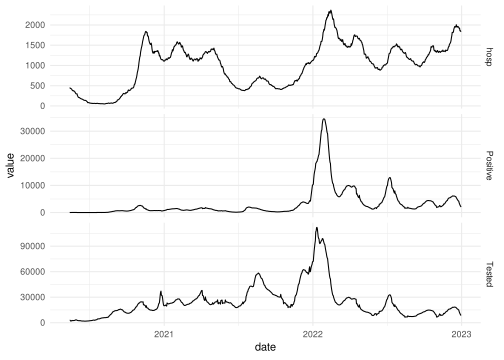
\includegraphics{template-computo-R_files/figure-pdf/covidintro-1.pdf}

}

\caption{Hospitalizations, IPTCC and positive PCR of Bordeaux University
Hospital.}

\end{figure}%

\subsubsection{First reservoir}\label{first-reservoir}

Setting a reservoir is done with the \texttt{createNode()} function. The
important hyperparameters are the following :

\begin{itemize}
\tightlist
\item
  Number of nodes (\texttt{units}) : it corresponds to the number of
  nodes inside the reservoir. Usually, the more the better, but more
  nodes increases the computation time.
\item
  Leaking rate (\texttt{lr}) : the leaking rate corresponds to the
  balance between the new inputs and the previous state. A leaking rate
  of 1 only consider information from new inputs.
\item
  Spectral radius (\texttt{sr}): the spectral radius is the maximum
  absolute eigenvalue of the reservoir connectivity matrix. A small
  spectral radius induces stable dynamics inside the reservoir, a high
  spectral radius induces a chaotic regime inside the reservoir.
\item
  Input scaling (\texttt{input\_scaling}): the input scaling is a gain
  applied to the input features of the reservoir.
\item
  Warmup (\texttt{warmup}) : it corresponds to the number of time step
  during which the data are propagating into the reservoir but not used
  to fit the output layer. This hyperparameter is set in the
  \texttt{reservoirR\_fit()} function.
\end{itemize}

In addition, we can set the seed (\texttt{seed}). Because the reservoir
connections are set at random, setting the seed is a good approach to
ensure reproducibility.

For this part of the tutorial, we will set the hyperparameter at a given
value. Hyperparameter optimization will be detailed at section
\hyperref[studycase]{Study case}.

Then we can feed the data to the reservoir and see the activation state
of the reservoir \(x(t)\). To do so, we first prepare the data and
transform it to a matrix:

Then we run the \texttt{predict\_seq} function. It takes as input a node
(i.e a reservoir or a reservoir associated with an output layer) and the
feature matrix.

Now we can visualize node activation using the \texttt{plot} function
presented at figure @ref(fig:nodeactivationbad).

\begin{figure}[H]

{\centering 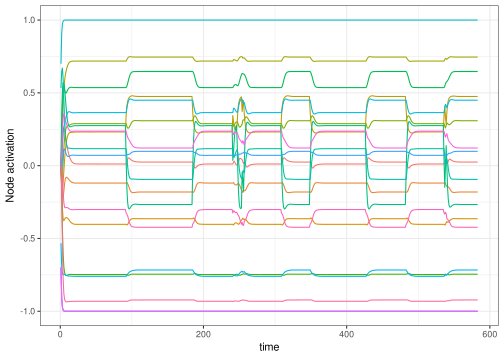
\includegraphics{template-computo-R_files/figure-pdf/nodeactivationbad-1.pdf}

}

\caption{20 random nodes activation over time.}

\end{figure}%

Numerous nodes within the system exhibit a consistent equilibrium state.
The challenge arises when the output layer attempts to extract knowledge
from these nodes, as they do not convey meaningful information. This
issue can be attributed to the disparate scales of the features. To
address this concern, a practical approach involves normalizing the
features by dividing each of them by their respective maximum values,
thereby scaling them within the range of \(-1\) to \(1\) by dividing by
the maximum of the absolute value. Of note, here the features will be
scaled between \(0\) and \(1\) because all features are positive.

We then feed them to the reservoir and plot the node activation again.
Compared to @ref(fig:nodeactivationbad), the obtained node activation
@ref(fig:nodeactivationgood) shows interesting trend outputs as no node
seems saturated.

\begin{figure}[H]

{\centering 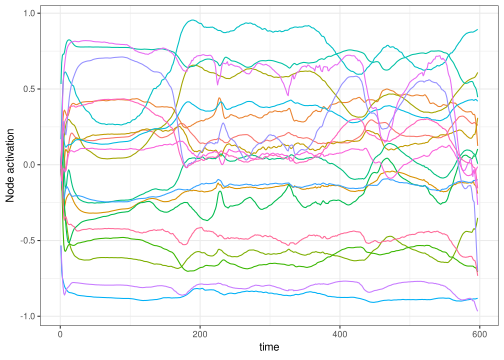
\includegraphics{template-computo-R_files/figure-pdf/nodeactivationgood-1.pdf}

}

\caption{20 random node activation over time. Scaled features.}

\end{figure}%

\subsubsection{Forecast}\label{forecast}

In order to train the reservoir, we should train the last layer which
linearly combines the neuron's output.

\paragraph{Set the ESN}\label{set-the-esn}

Initially, we establish the output layer, incorporating a ridge penalty
set at \texttt{1e3}. It's important to note that this hyperparameter can
be subject to optimization, a topic that will be explored in the
forthcoming \hyperref[studycase]{Study Case} section. This parameter
plays a pivotal role in fine-tuning the model's conformity to the data.
When set excessively high, the risk of underfitting arises, whereas
setting it too low can lead to overfitting. We connect the output layer
to the reservoir making the model ready to be trained.

\paragraph{Set the data}\label{set-the-data}

First we separate the train set on which we will learn the ridge
coefficients and the test set on which we will make the forecast. We
define the train set to be all the data before 2022-01-01 and the test
data to be all the data to have forecast both on train and test sets.

We standardize with the same formula as seen before. We learn the
standardization on the training set and apply it on the test set. Then
we convert the dataframe to matrix.

\paragraph{Train the model and
predict}\label{train-the-model-and-predict}

We then feed the reservoir with the train set. To do so, we set a
\texttt{warmup} of \texttt{30} days during which the data are
propagating into the reservoir but not used to fit the output layer.

Now that the ridge layer is trained, we can forecast. We set the
parameter \texttt{reset} to \texttt{TRUE} in order to clean the
reservoir from the data used by the training set.

\begin{figure}[H]

{\centering 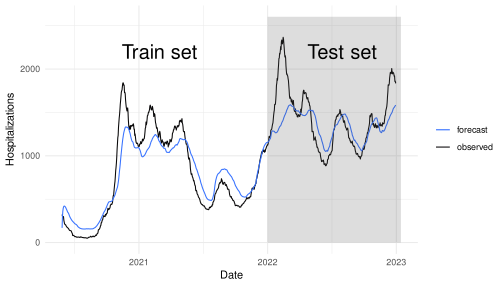
\includegraphics{template-computo-R_files/figure-pdf/unnamed-chunk-13-1.pdf}

}

\caption{Forecast}

\end{figure}%

We observe that the model forecast is not fully accurate, both on the
test set and the train set. In that case, one option could be to reduce
ridge penalization to fit more closely the data, the optimization of
ridge hyperparameter will be discussed at section
\hyperref[studycase]{Study case}. Another possibility is to ease the
learning of the algorithm by forecasting the variation of the
hospitalization instead of the number of hospitalized patients. For that
step, we will learn on the \texttt{outcome\_deriv} contained in
\texttt{yTrain\_variation} data which is defined outcome as
\texttt{outcome\_deriv\ =\ outcome\ -\ hosp}. As depicted at figure
@ref(fig:figForecastDerivvsRaw), this strategy improved the model
forecast.

\begin{figure}[H]

{\centering 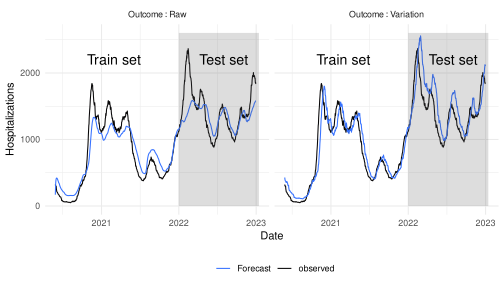
\includegraphics{template-computo-R_files/figure-pdf/figForecastDerivvsRaw-1.pdf}

}

\caption{Covid-19 hospitalizations forecast. The model is either trained
to forecast the number of hospitalizations (denoted Raw) or the
variation of the hospitalizations compared to current level of
hospitalisation (denoted Variation)}

\end{figure}%

\subsection{Classification}\label{classification}

\subsubsection{The Japanese vowel
dataset}\label{the-japanese-vowel-dataset}

This example is largely inspired from the
\href{https://github.com/reservoirpy/reservoirpy/blob/master/tutorials/5-Classification-with-RC.ipynb}{classification
tutorial of reservoirpy}. To illustrate the classification task, we will
use the Japanese vowel dataset (Kudo, Toyama, and Shimbo (1999)). The
data can be loaded from \texttt{reservoirnet} as follow :

The dataset comprises 640 vocalizations of the Japanese vowel \ae,
contributed by nine distinct speakers. Each vocalization represents a
time series spanning between 7 and 29 time steps, encoded as a
12-dimensional vector denoting the Linear Prediction Coefficients (LPC).
A visual representation of six distinct utterances from the test set,
originating from three different speakers, is depicted in Figure
@ref(fig:vowelpresentation).

\begin{figure}[H]

{\centering 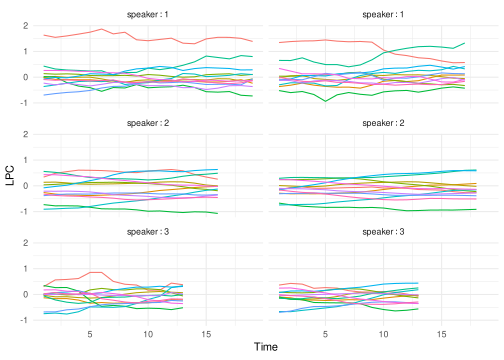
\includegraphics{template-computo-R_files/figure-pdf/vowelpresentation-1.pdf}

}

\caption{Vowel dataset, sample with 3 speakers and 2 utterance each.}

\end{figure}%

The primary objective involves the attribution of each utterance to its
respective speaker, this is denoted as classification or
sequence-to-vector encoding. The secondary objective involves the
attribution of each time step of each utterance to its speaker, this is
denoted as transduction or sequence-to-sequence encoding.

\subsubsection{Classification (sequence-to-vector
model)}\label{classification-sequence-to-vector-model}

The first approach is the sequence-to-vector encoding. For this task we
aim to predict the speaker of the whole utterance (i.e the label is
assigned to the whole sequence). We first start by creating the
reservoir and the output layer.

To perform this task, we need to modify the training and testing
processes. Leveraging the inherent inertia of the reservoir, information
from preceding time steps is preserved, effectively endowing the RC with
a form of memory. Consequently, the final state vector encapsulates
insights gathered from all antecedent states. In the context of the
sequence-to-vector encoding task, only this ultimate state is employed.
This process is executed as follows:

\emph{XH : Markovian or ``echo state'' property ? c'est pour dire que
les états finissent par être oubliés au bout d'un certain temps, donc
c'est pas ce que tu veux dire là je pense}

\emph{TF : j'ai remplacé par inertia qui parait effectivement plus
approprié. Mon idée c'est que l'information s'accumule dans le réservoir
au fur et à mesure qu'il ``lit'' la séquence de données.}

Then we can train the readout based on this last state vector. In that
case, \texttt{Y\_train} contains a single label for each utterance.

The prediction is also modified using only the final state :

Figure @ref(fig:seqtovec) shows the prediction for the 6 utterances
depicted at figure @ref(fig:vowelpresentation) where the model correctly
identifies the speaker.

\begin{figure}[H]

{\centering 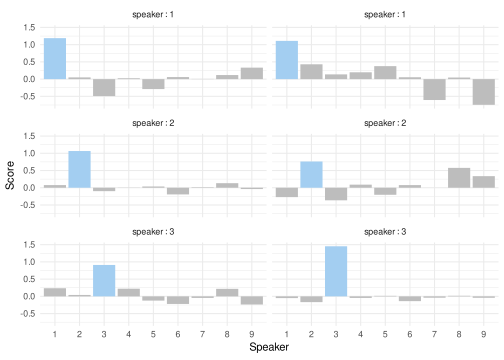
\includegraphics{template-computo-R_files/figure-pdf/seqtovec-1.pdf}

}

\caption{Prediction in a sequence-to-sequence approach 6 samples with 3
speakers and 2 utterance each. The speaker to predict is depicted in
blue. For each of the 6 utterance, the model correctly identifies the
speaker.}

\end{figure}%

Then, we can also compute the overall accuracy :

\begin{verbatim}
[1] "Accuracy: 92.703%"
\end{verbatim}

\subsubsection{Transduction (sequence-to-sequence
model)}\label{transduction-sequence-to-sequence-model}

For this task, the goal is to predict the speaker for each time step of
each utterance. The first step is to get the data where the label is
repeated for each time step. This is easily done with the
\texttt{repeat\_targets} argument as follow :

Then we can train a simple Echo State Network to solve this task. For
this example we will connect both the input layer and the reservoir
layer to the readout layer which is performed by the
\texttt{\%\textgreater{}\textgreater{}\%} operator :

We can then fit the model and predict the labels for the test data. The
\texttt{reset} parameter is set to \texttt{TRUE} to remove information
from the reservoir from the training process.

From the \texttt{Y\_pred} and \texttt{Y\_test} we represent at figure
@ref(fig:figseqtoseq) the predictions for the same patients as in figure
@ref(fig:vowelpresentation).

\begin{figure}[H]

{\centering 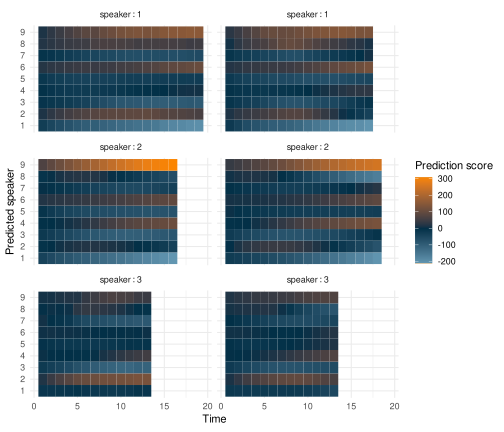
\includegraphics{template-computo-R_files/figure-pdf/figseqtoseq-1.pdf}

}

\caption{Prediction in a sequence-to-sequence approach 6 samples with 3
speakers and 2 utterance each. The higher the score of the speaker, the
lighter the color.}

\end{figure}%

For those 6 utterances, the model correctly identify the speaker for
most of the time steps. We can then evaluate the overall accuracy of the
model :

\begin{verbatim}
[1] "Accuracy: 92.456%"
\end{verbatim}

\section{Introduction}\label{introduction-1}

\subsection{About this document}\label{about-this-document}

This document, accompanied with the
\href{https://github.com/computorg/template-computo-R/}{hopefully finely
tuned git repos}, provides a template for writing contributions to
\textbf{Computo} (\textbf{computo?}). We show how \texttt{R} code
(\textbf{R-base?}) can be included and how the repository can be set up
for triggering github actions for rendering the document, with
dependencies handled by \texttt{renv}.

\subsection{Setup a github repository for preparing your
submission}\label{setup-a-github-repository-for-preparing-your-submission}

You can start by clicking the \textbf{``use this template''} button, on
the top of the page of the
\href{https://github.com/computorg/template-computo-R/}{github
repository associated to this document}. Of course, you can set your
repository private during the preparation of your manuscript.

\subsection{Quarto}\label{quarto}

\href{https://quarto.org/}{Quarto} is a versatile formatting system for
authoring documents integrating markdown, LaTeX and code blocks
interpreted either via Jupyter or Knitr (thus supporting Python, R and
Julia). It relies on the \href{https://pandoc.org/MANUAL.html}{Pandoc}
document converter.

\subsection{Requirements}\label{requirements}

You need \href{https://quarto.org/}{quarto} installed on your system and
the \href{https://github.com/computorg/computo-quarto-extension}{Computo
extension} to prepare your document. For the latter, once quarto is
installed, run the following to install the extension in the current
directory (it creates a \texttt{\_extension} directory which is ignored
by git thanks to \texttt{.gitignore} by default):

\begin{Shaded}
\begin{Highlighting}[]
\ExtensionTok{quarto}\NormalTok{ add computorg/computo{-}quarto{-}extension}
\end{Highlighting}
\end{Shaded}

\href{https://www.r-project.org/}{\texttt{R}} and the following
\texttt{R} packages must be installed on your computer:
\href{https://cran.r-project.org/package=knitr}{\texttt{knitr}},
\href{https://cran.r-project.org/package=markdown}{\texttt{markdown}}.

\subsection{Link with your usual
tools}\label{link-with-your-usual-tools}

Quarto is expecting a \texttt{.qmd} markdown file, but will also works
with a standard
\href{https://rmarkdown.rstudio.com/}{\texttt{Rmarkdown}}
(\texttt{.Rmd}) file. In addition, especially if you are not comfortable
with the command line interface, quarto is fully integrated inside the
\href{https://quarto.org/docs/get-started/hello/rstudio.html}{Rstudio
IDE} so that you can write and build your quarto document inside
Rstudio.

Quarto can also process a
\href{https://quarto.org/docs/get-started/hello/jupyter.html}{Jupyter
notebook} file if you are used to it (it will just require to add the
proper YAML metadata\footnote{the same metadata as in the
  \href{https://github.com/computorg/template-computo-R/blob/main/template-computo-R.qmd}{\texttt{template-computo-R.qmd}
  file} in the first cell, type ``Raw'', of the notebook}).

\textbf{Note}: \emph{More advanced Jupyter-related functionality like
Myst/Jupyter book are not supported in this Quarto setup. The markdown
syntax inside the Jupyter notebook should follow the Quarto syntax (c.f.
\hyperref[formatting]{below}). If you are more comfortable with using
Myst/Jupyter book, we provide a
\href{https://github.com/computorg/template-computo-myst}{specific
template} but it will requires more formatting work for Computo
editorial team, thus highly encourage authors to use the Quarto
templates.}

\section{Formatting}\label{formatting}

This section covers basic formatting guidelines for quarto documents.

To render a document, run \texttt{quarto\ render}. By default, both PDF
and HTML documents are generated:

\begin{Shaded}
\begin{Highlighting}[]
\ExtensionTok{quarto}\NormalTok{ render template{-}computo{-}R.qmd }\CommentTok{\# will render both to html and PDF}
\end{Highlighting}
\end{Shaded}

\begin{tcolorbox}[enhanced jigsaw, breakable, toptitle=1mm, arc=.35mm, bottomtitle=1mm, colback=white, colframe=quarto-callout-tip-color-frame, opacitybacktitle=0.6, colbacktitle=quarto-callout-tip-color!10!white, opacityback=0, toprule=.15mm, leftrule=.75mm, left=2mm, title=\textcolor{quarto-callout-tip-color}{\faLightbulb}\hspace{0.5em}{Note}, rightrule=.15mm, titlerule=0mm, bottomrule=.15mm, coltitle=black]

To check the syntax of the formatting below, you can use the
\texttt{\textless{}/\textgreater{}\ source} button at the top left of
this document.

\end{tcolorbox}

\subsection{Basic markdown formatting}\label{basic-markdown-formatting}

\textbf{Bold text} or \emph{italic}

\begin{itemize}
\tightlist
\item
  This is a list
\item
  With more elements
\item
  It isn't numbered.
\end{itemize}

But we can also do a numbered list

\begin{enumerate}
\def\labelenumi{\arabic{enumi}.}
\tightlist
\item
  This is my first item
\item
  This is my second item
\item
  This is my third item
\end{enumerate}

\subsection{Mathematics}\label{mathematics}

\subsubsection{Mathematical formulae}\label{mathematical-formulae}

\href{https://www.latex-project.org/}{LaTeX} code is natively
supported\footnote{We use \href{https://lualatex.org/}{lualatex} for
  this purpose.}, which makes it possible to use mathematical formulae:

\[
f(x_1, \dots, x_n; \mu, \sigma^2) =
\frac{1}{\sigma \sqrt{2\pi}} \exp{\left(- \frac{1}{2\sigma^2}\sum_{i=1}^n(x_i - \mu)^2\right)}
\]

It is also posible to cross-reference an equation, see
Equation~\ref{eq-mylabel}:

\begin{equation}\phantomsection\label{eq-mylabel}{
\begin{aligned}
D_{x_N} & = \frac12
\left[\begin{array}{cc}
x_L^\top & x_N^\top \end{array}\right] \,
\left[\begin{array}{cc}  L_L & B \\ B^\top & L_N \end{array}\right] \,
\left[\begin{array}{c}
x_L \\ x_N \end{array}\right] \\
& = \frac12 (x_L^\top L_L x_L + 2 x_N^\top B^\top x_L + x_N^\top L_N x_N),
\end{aligned}
}\end{equation}

\subsubsection{Theorems and other amsthem-like
environments}\label{theorems-and-other-amsthem-like-environments}

Quarto includes a nice support for theorems, with predefined prefix
labels for theorems, lemmas, proposition, etc. see
\href{https://quarto.org/docs/authoring/cross-references.html\#theorems-and-proofs}{this
page}. Here is a simple example:

\begin{theorem}[Strong law of large
numbers]\protect\hypertarget{thm-slln}{}\label{thm-slln}

The sample average converges almost surely to the expected value:

\[\overline{X}_n\ \xrightarrow{\text{a.s.}}\ \mu \qquad\textrm{when}\ n \to \infty.\]

\end{theorem}

See Theorem~\ref{thm-slln}.

\subsection{R Code}\label{r-code}

Quarto uses either Jupyter or knitr to render code chunks. This can be
triggered in the yaml header. In this tutorial, we use \texttt{knitr}
(\texttt{R} and packages \texttt{knitr}, \texttt{markdown} must be
installed on your computer).

\begin{Shaded}
\begin{Highlighting}[]
\PreprocessorTok{{-}{-}{-}}
\FunctionTok{title}\KeywordTok{:}\AttributeTok{ }\StringTok{"My Document"}
\AttributeTok{author "Jane Doe"}
\PreprocessorTok{{-}{-}{-}}
\end{Highlighting}
\end{Shaded}

\texttt{R} code (\textbf{R-base?}) chunks may be embedded as follows:

\begin{Shaded}
\begin{Highlighting}[]
\NormalTok{x }\OtherTok{\textless{}{-}} \FunctionTok{rnorm}\NormalTok{(}\DecValTok{10}\NormalTok{)}
\end{Highlighting}
\end{Shaded}

\subsection{Figures}\label{figures}

Plots can be generated as follows:

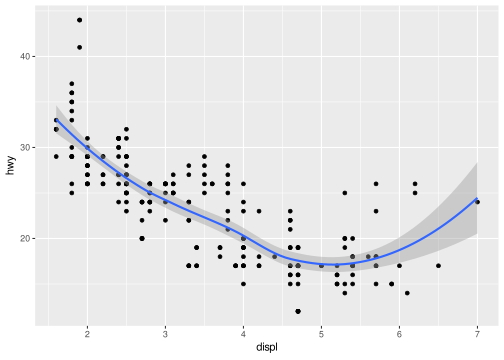
\includegraphics{template-computo-R_files/figure-pdf/pressure-1.pdf}

It is also possible to create figures from static images:

\begin{figure}

\centering{

\includegraphics[width=\textwidth,height=2.08333in]{template-computo-R_files/mediabag/logo_text_vertical.png}

}

\caption{\label{fig-logo}Computo logo (label)}

\end{figure}%

\textbf{Note:} \emph{Until Quarto version 1.3+ is released, including a
remote image (from a web URL) in a document (like the image above) will
work in the rendered HTML document but will generate an error when
building the PDF document (c.f.
\href{https://github.com/quarto-dev/quarto-cli/issues/4443}{related bug
report}).}

\subsection{Tables}\label{tables}

Tables (with label: \texttt{@tbl-mylabel} renders
Table~\ref{tbl-mylabel}) can be generated with markdown as follows

\begin{longtable}[]{@{}lcr@{}}
\caption{my table caption}\label{tbl-mylabel}\tabularnewline
\toprule\noalign{}
Tables & Are & Cool \\
\midrule\noalign{}
\endfirsthead
\toprule\noalign{}
Tables & Are & Cool \\
\midrule\noalign{}
\endhead
\bottomrule\noalign{}
\endlastfoot
col 1 is & left-aligned & \$1600 \\
col 2 is & centered & \$12 \\
col 3 is & right-aligned & \$1 \\
\end{longtable}

Table can also be generated by some code, for instance with knitr here:

\begin{longtable}[]{@{}lll@{}}
\caption{Table caption.}\tabularnewline
\toprule\noalign{}
& speed & dist \\
\midrule\noalign{}
\endfirsthead
\toprule\noalign{}
& speed & dist \\
\midrule\noalign{}
\endhead
\bottomrule\noalign{}
\endlastfoot
& Min. : 4.0 & Min. : 2.00 \\
& 1st Qu.:12.0 & 1st Qu.: 26.00 \\
& Median :15.0 & Median : 36.00 \\
& Mean :15.4 & Mean : 42.98 \\
& 3rd Qu.:19.0 & 3rd Qu.: 56.00 \\
& Max. :25.0 & Max. :120.00 \\
\end{longtable}

\subsection{Handling references}\label{sec-references}

\subsubsection{Bibliographic references}\label{bibliographic-references}

References are displayed as footnotes using
\href{http://www.bibtex.org/}{BibTeX}, e.g.~\texttt{{[}@computo{]}} will
be displayed as (\textbf{computo?}), where \texttt{computo} is the
bibtex key for this specific entry. The bibliographic information is
automatically retrieved from the \texttt{.bib} file specified in the
header of this document (here: \texttt{references.bib}).

\subsubsection{Other cross-references}\label{other-cross-references}

As already (partially) seen, Quarto includes a mechanism similar to the
bibliographic references for sections, equations, theorems, figures,
lists, etc. Have a look at
\href{https://quarto.org/docs/authoring/cross-references.html}{this
page}.

\subsection{Advanced formatting}\label{advanced-formatting}

Advanced formatting features are possible and documented (including
interactive plots, pseudo-code, (Tikz) diagrams, Lua filters, mixing R +
Python in the same document), but are beyond the scope of this simple
introduction. We point several entries in this direction.

\begin{tcolorbox}[enhanced jigsaw, breakable, toptitle=1mm, arc=.35mm, bottomtitle=1mm, colback=white, colframe=quarto-callout-warning-color-frame, opacitybacktitle=0.6, colbacktitle=quarto-callout-warning-color!10!white, opacityback=0, toprule=.15mm, leftrule=.75mm, left=2mm, title=\textcolor{quarto-callout-warning-color}{\faExclamationTriangle}\hspace{0.5em}{More information}, rightrule=.15mm, titlerule=0mm, bottomrule=.15mm, coltitle=black]

\begin{itemize}
\item
  \href{https://quarto.org}{The Quarto web site} for comprehensive
  documentation, including:

  \begin{itemize}
  \tightlist
  \item
    \href{https://quarto.org/docs/get-started/}{Tutorial}
  \item
    \href{https://quarto.org/docs/guide/}{User guide}
  \item
    \href{https://quarto.org/docs/reference/}{Options reference}
  \end{itemize}
\item
  \href{https://computo.sfds.asso.fr/computo-quarto-extension/}{The
  template distributed with the Computo Quarto extension}, which uses
  such advanced features.
\item
  \href{https://computo.sfds.asso.fr/published-paper-tsne/}{Our mock
  version of the t-SNE paper}, a full and advanced example using Python
  and the Jupyter kernel.
\item
  \href{https://computo.sfds.asso.fr/publications/}{The previously
  published papers in Computo} can be used as references.
\end{itemize}

\end{tcolorbox}

\section{Finalize your submission}\label{finalize-your-submission}

\subsection{\texorpdfstring{Handle \texttt{R} dependencies with
\texttt{renv}}{Handle R dependencies with renv}}\label{handle-r-dependencies-with-renv}

To make your work reproducible, you need to fix the packages and
environment used to run your analysis. For the \texttt{R} system, the
\texttt{renv} package is one of the possible reliable method, supported
by the community. You basically need a couple of commands to setup your
environment on your local machine. First,

will initialize your repository. Then you just need to install the
dependencies required to run your contribution, for instance,

Non-CRAN packages (\emph{e.g.} Github packages) can be used. Once you
are done, you can fix everything with the command

\begin{tcolorbox}[enhanced jigsaw, breakable, toptitle=1mm, arc=.35mm, bottomtitle=1mm, colback=white, colframe=quarto-callout-important-color-frame, opacitybacktitle=0.6, colbacktitle=quarto-callout-important-color!10!white, opacityback=0, toprule=.15mm, leftrule=.75mm, left=2mm, title=\textcolor{quarto-callout-important-color}{\faExclamation}\hspace{0.5em}{Important}, rightrule=.15mm, titlerule=0mm, bottomrule=.15mm, coltitle=black]

The only file that needs to be versioned by git is \texttt{renv.lock}.
By default, the rest is ignored thanks to \texttt{.gitignore}.

\end{tcolorbox}

More details for using \texttt{renv} can be found either

\begin{itemize}
\tightlist
\item
  on the
  \href{https://rstudio.github.io/renv/articles/renv.html}{\texttt{renv}
  packge webpage}, or
\item
  on the
  \href{https://quarto.org/docs/projects/virtual-environments.html\#using-renv}{quarto
  page dedicated to environments}
\end{itemize}

\subsection{Continuous integration}\label{continuous-integration}

The repository associated with this template is pre-configure to trigger
an action on push that performs the following:

\begin{enumerate}
\def\labelenumi{\arabic{enumi}.}
\tightlist
\item
  Check out repository on the \texttt{ubuntu-latest} machine
\item
  Install quarto and dependencies, including the Computo extension
\item
  Install R and dependencies with \texttt{renv}, using your
  \texttt{renv.lock} file
\item
  Render your .qmd file and Publish the results on a gh-page (both HTML
  and PDF)
\end{enumerate}

The file
\href{https://github.com/computorg/template-computo-R/blob/main/.github/workflows/build.yml}{.github/workflows/build.yml}
is largely inspired from
\href{https://quarto.org/docs/publishing/github-pages.html\#example-knitr-with-renv}{this
file}.

Once this is successful, you are ready to submit your manuscript to the
\href{https://computo.scholasticahq.com/}{Computo submission platform}.

\begin{tcolorbox}[enhanced jigsaw, breakable, toptitle=1mm, arc=.35mm, bottomtitle=1mm, colback=white, colframe=quarto-callout-warning-color-frame, opacitybacktitle=0.6, colbacktitle=quarto-callout-warning-color!10!white, opacityback=0, toprule=.15mm, leftrule=.75mm, left=2mm, title=\textcolor{quarto-callout-warning-color}{\faExclamationTriangle}\hspace{0.5em}{Warning}, rightrule=.15mm, titlerule=0mm, bottomrule=.15mm, coltitle=black]

The first time, you possibly need to create the branch for the action to
work. This can be done by running the following command from your
computer, in your git repository:

\begin{Shaded}
\begin{Highlighting}[]
\ExtensionTok{quarto}\NormalTok{ publish gh{-}pages}
\end{Highlighting}
\end{Shaded}

Then, set the branch \texttt{gh-page} as the source of your github page,
and trigger the action to check that everything works fine.

\end{tcolorbox}

\subsection{Data and large files}\label{data-and-large-files}

If your submission materials contain files larger\,than 50MB,
\textbf{especially data files}, they won't fit on a git repository as
is. For this reason, we encourage\,you to put your data or any materials
you\,deem necessary on an external ``open data'' centered\,repository
hub such a \href{https://zenodo.org/}{Zenodo} or
\href{https://osf.io/}{OSF}.

\section*{References}\label{references}
\addcontentsline{toc}{section}{References}

\phantomsection\label{refs}
\begin{CSLReferences}{1}{0}
\bibitem[\citeproctext]{ref-hinaut_real-time_2013}
Hinaut, Xavier, and Peter Ford Dominey. 2013. {``Real-{Time} {Parallel}
{Processing} of {Grammatical} {Structure} in the {Fronto}-{Striatal}
{System}: {A} {Recurrent} {Network} {Simulation} {Study} {Using}
{Reservoir} {Computing}.''} \emph{PLOS ONE} 8 (2): e52946.
\url{https://doi.org/10.1371/journal.pone.0052946}.

\bibitem[\citeproctext]{ref-jaeger__2001}
Jaeger, Herbert. 2001. {``The" Echo State" Approach to Analysing and
Training Recurrent Neural Networks-with an Erratum Note'.''} \emph{Bonn,
Germany: German National Research Center for Information Technology GMD
Technical Report} 148 (January).

\bibitem[\citeproctext]{ref-kudo_multidimensional_1999}
Kudo, Mineichi, Jun Toyama, and Masaru Shimbo. 1999. {``Multidimensional
Curve Classification Using Passing-Through Regions.''} \emph{Pattern
Recognition Letters} 20 (11): 1103--11.
\url{https://doi.org/10.1016/S0167-8655(99)00077-X}.

\bibitem[\citeproctext]{ref-lukosevicius_reservoir_2009}
Lukoševičius, Mantas, and Herbert Jaeger. 2009. {``Reservoir Computing
Approaches to Recurrent Neural Network Training.''} \emph{Computer
Science Review} 3 (3): 127--49.
\url{https://doi.org/10.1016/j.cosrev.2009.03.005}.

\bibitem[\citeproctext]{ref-maass_real-time_2002}
Maass, Wolfgang, Thomas Natschläger, and Henry Markram. 2002.
{``Real-Time Computing Without Stable States: A New Framework for Neural
Computation Based on Perturbations.''} \emph{Neural Computation} 14
(11): 2531--60. \url{https://doi.org/10.1162/089976602760407955}.

\bibitem[\citeproctext]{ref-martinuzzi_reservoircomputingjl_2022}
Martinuzzi, Francesco, Chris Rackauckas, Anas Abdelrehim, Miguel D.
Mahecha, and Karin Mora. 2022. {``{ReservoirComputing}.jl: {An}
{Efficient} and {Modular} {Library} for {Reservoir} {Computing}
{Models}.''} \emph{Journal of Machine Learning Research} 23 (288): 1--8.
\url{http://jmlr.org/papers/v23/22-0611.html}.

\bibitem[\citeproctext]{ref-nakane_reservoir_2018}
Nakane, Ryosho, Gouhei Tanaka, and Akira Hirose. 2018. {``Reservoir
{Computing} {With} {Spin} {Waves} {Excited} in a {Garnet} {Film}.''}
\emph{IEEE Access} PP (January): 1--1.
\url{https://doi.org/10.1109/ACCESS.2018.2794584}.

\bibitem[\citeproctext]{ref-pedersen_patchwork_2023}
Pedersen, Thomas Lin. 2023. {``Patchwork: {The} {Composer} of
{Plots}.''}
\href{https://patchwork.data-imaginist.com,\%20https://github.com/thomasp85/patchwork}{https://patchwork.data-imaginist.com,
https://github.com/thomasp85/patchwork}.

\bibitem[\citeproctext]{ref-penkovsky_efficient_2018}
Penkovsky, Bogdan, Laurent Larger, and Daniel Brunner. 2018.
{``Efficient Design of Hardware-Enabled Reservoir Computing in
{FPGAs}.''} \emph{Journal of Applied Physics} 124 (16): 162101.
\url{https://doi.org/10.1063/1.5039826}.

\bibitem[\citeproctext]{ref-prychynenko_magnetic_2018}
Prychynenko, Diana, Matthias Sitte, Kai Litzius, Benjamin Krüger, George
Bourianoff, Mathias Kläui, Jairo Sinova, and Karin Everschor-Sitte.
2018. {``Magnetic {Skyrmion} as a {Nonlinear} {Resistive} {Element}: {A}
{Potential} {Building} {Block} for {Reservoir} {Computing}.''}
\emph{Physical Review Applied} 9 (1): 014034.
\url{https://doi.org/10.1103/PhysRevApplied.9.014034}.

\bibitem[\citeproctext]{ref-rafayelyan_large-scale_2020}
Rafayelyan, Mushegh, Jonathan Dong, Yongqi Tan, Florent Krzakala, and
Sylvain Gigan. 2020. {``Large-{Scale} {Optical} {Reservoir} {Computing}
for {Spatiotemporal} {Chaotic} {Systems} {Prediction}.''} \emph{Physical
Review X} 10 (4): 041037.
\url{https://doi.org/10.1103/PhysRevX.10.041037}.

\bibitem[\citeproctext]{ref-tanaka_recent_2019}
Tanaka, Gouhei, Toshiyuki Yamane, Jean Benoit Héroux, Ryosho Nakane,
Naoki Kanazawa, Seiji Takeda, Hidetoshi Numata, Daiju Nakano, and Akira
Hirose. 2019. {``Recent Advances in Physical Reservoir Computing: {A}
Review.''} \emph{Neural Networks} 115 (July): 100--123.
\url{https://doi.org/10.1016/j.neunet.2019.03.005}.

\bibitem[\citeproctext]{ref-trouvain_canary_2021}
Trouvain, Nathan, and Xavier Hinaut. 2021. {``Canary {Song} {Decoder}:
{Transduction} and {Implicit} {Segmentation} with {ESNs} and {LTSMs}.''}
In \emph{Artificial {Neural} {Networks} and {Machine} {Learning} --
{ICANN} 2021}, edited by Igor Farkaš, Paolo Masulli, Sebastian Otte, and
Stefan Wermter, 71--82. Lecture {Notes} in {Computer} {Science}. Cham:
Springer International Publishing.
\url{https://doi.org/10.1007/978-3-030-86383-8_6}.

\bibitem[\citeproctext]{ref-trouvain_reservoirpy_2022}
---------. 2022. {``Reservoirpy: {A} {Simple} and {Flexible} {Reservoir}
{Computing} {Tool} in {Python}.''}
\url{https://inria.hal.science/hal-03699931}.

\bibitem[\citeproctext]{ref-trouvain_reservoirpy_2020}
Trouvain, Nathan, Luca Pedrelli, Thanh Trung Dinh, and Xavier Hinaut.
2020. {``{ReservoirPy}: An {Efficient} and {User}-{Friendly} {Library}
to {Design} {Echo} {State} {Networks}.''} In.
\url{https://inria.hal.science/hal-02595026}.

\bibitem[\citeproctext]{ref-trouvain_create_2022}
Trouvain, Nathan, Nicolas Rougier, and Xavier Hinaut. 2022. {``Create
{Efficient} and~{Complex} {Reservoir} {Computing} {Architectures}
with~{ReservoirPy}.''} In \emph{From {Animals} to {Animats} 16}, edited
by Lola Cañamero, Philippe Gaussier, Myra Wilson, Sofiane Boucenna, and
Nicolas Cuperlier, 91--102. Lecture {Notes} in {Computer} {Science}.
Cham: Springer International Publishing.
\url{https://doi.org/10.1007/978-3-031-16770-6_8}.

\bibitem[\citeproctext]{ref-vlachas_backpropagation_2020}
Vlachas, P. R., J. Pathak, B. R. Hunt, T. P. Sapsis, M. Girvan, E. Ott,
and P. Koumoutsakos. 2020. {``Backpropagation Algorithms and {Reservoir}
{Computing} in {Recurrent} {Neural} {Networks} for the Forecasting of
Complex Spatiotemporal Dynamics.''} \emph{Neural Networks} 126 (June):
191--217. \url{https://doi.org/10.1016/j.neunet.2020.02.016}.

\bibitem[\citeproctext]{ref-wickham_ggplot2_2016}
Wickham, Hadley. 2016. \emph{Ggplot2: {Elegant} {Graphics} for {Data}
{Analysis}}. Springer-Verlag New York.
\url{https://ggplot2.tidyverse.org}.

\bibitem[\citeproctext]{ref-wickham_dplyr_2023}
Wickham, Hadley, Romain François, Lionel Henry, Kirill Müller, and Davis
Vaughan. 2023. {``Dplyr: {A} {Grammar} of {Data} {Manipulation}.''}
\url{https://CRAN.R-project.org/package=dplyr}.

\end{CSLReferences}

\section*{Session information}\label{session-information}
\addcontentsline{toc}{section}{Session information}

\begin{verbatim}
R version 4.2.2 Patched (2022-11-10 r83330)
Platform: x86_64-pc-linux-gnu (64-bit)
Running under: Ubuntu 20.04.6 LTS

Matrix products: default
BLAS:   /usr/lib/x86_64-linux-gnu/blas/libblas.so.3.9.0
LAPACK: /usr/lib/x86_64-linux-gnu/lapack/liblapack.so.3.9.0

locale:
 [1] LC_CTYPE=fr_FR.UTF-8       LC_NUMERIC=C              
 [3] LC_TIME=fr_FR.UTF-8        LC_COLLATE=fr_FR.UTF-8    
 [5] LC_MONETARY=fr_FR.UTF-8    LC_MESSAGES=fr_FR.UTF-8   
 [7] LC_PAPER=fr_FR.UTF-8       LC_NAME=C                 
 [9] LC_ADDRESS=C               LC_TELEPHONE=C            
[11] LC_MEASUREMENT=fr_FR.UTF-8 LC_IDENTIFICATION=C       

attached base packages:
[1] stats     graphics  grDevices datasets  utils     methods   base     

other attached packages:
[1] reservoirnet_0.2.0 patchwork_1.1.3    ggplot2_3.5.1      dplyr_1.1.2       

loaded via a namespace (and not attached):
 [1] Rcpp_1.0.10      lubridate_1.9.2  here_1.0.1       lattice_0.20-45 
 [5] tidyr_1.3.0      png_0.1-8        rprojroot_2.0.3  digest_0.6.33   
 [9] utf8_1.2.3       R6_2.5.1         backports_1.4.1  evaluate_0.20   
[13] pillar_1.9.0     rlang_1.1.4      car_3.1-1        Matrix_1.5-1    
[17] reticulate_1.28  rmarkdown_2.20   slider_0.3.0     labeling_0.4.2  
[21] splines_4.2.2    stringr_1.5.0    munsell_0.5.0    broom_1.0.5     
[25] compiler_4.2.2   janitor_2.2.0    xfun_0.37        pkgconfig_2.0.3 
[29] mgcv_1.8-41      htmltools_0.5.4  tidyselect_1.2.0 tibble_3.2.1    
[33] fansi_1.0.4      withr_2.5.0      ggpubr_0.6.0     brio_1.1.3      
[37] rappdirs_0.3.3   grid_4.2.2       nlme_3.1-162     jsonlite_1.8.4  
[41] gtable_0.3.1     lifecycle_1.0.3  magrittr_2.0.3   scales_1.3.0    
[45] warp_0.2.0       cli_3.6.1        stringi_1.7.12   carData_3.0-5   
[49] farver_2.1.1     renv_1.0.11      ggsignif_0.6.4   testthat_3.1.7  
[53] snakecase_0.11.0 generics_0.1.3   vctrs_0.6.3      tools_4.2.2     
[57] glue_1.6.2       purrr_1.0.2      abind_1.4-5      fastmap_1.1.1   
[61] yaml_2.3.7       timechange_0.2.0 colorspace_2.1-0 rstatix_0.7.2   
[65] knitr_1.42      
\end{verbatim}




\end{document}
